\documentclass{report}

\input{preamble}
\input{macros}
\input{letterfonts}

\usepackage{tikz}
\usepackage{tikz-3dplot}
\usepackage{amsmath}
\usepackage{pgfplots}
\usepackage{smartdiagram}
\usesmartdiagramlibrary{additions}
\usepackage{xcolor}
\usepackage{forest}
\usetikzlibrary{circuits.logic.US} % Load the correct library for US-style logic gates
\usepgfplotslibrary{colormaps}
\usepgfplotslibrary{groupplots}
\usepgfplotslibrary{polar}
\pgfplotsset{compat=newest}
\tikzset{>=latex}
\usepackage{siunitx}

\title{\Huge{Intro to Software Engineering}\\EK327}
\author{\huge{Giacomo Cappelletto}}
\date{21/1/25}

\begin{document}


\maketitle
\newpage
\pdfbookmark[section]{\contentsname}{toc}
\tableofcontents
\pagebreak

\chapter{Computer Architecture}

\section{Adding Two Single-Bit Binaries Using XOR and AND Gates}

To add two single-bit binary numbers \( A \) and \( B \), we need to calculate:
1. The \textbf{sum bit}, which is the XOR of \( A \) and \( B \).
2. The \textbf{carry bit}, which is the AND of \( A \) and \( B \).

\textbf{Logic}
- \textbf{Sum Bit:} \( \text{Sum} = A \oplus B \)
- \textbf{Carry Bit:} \( \text{Carry} = A \cdot B \)

\bigskip

The following truth table summarizes the operation:

\[
	\begin{array}{|c|c|c|c|}
		\hline
		A & B & \text{Sum} & \text{Carry} \\
		\hline
		0 & 0 & 0          & 0            \\
		0 & 1 & 1          & 0            \\
		1 & 0 & 1          & 0            \\
		1 & 1 & 0          & 1            \\
		\hline
	\end{array}
\]

\bigskip

The addition is implemented using XOR and AND gates as shown below:

\begin{center}
	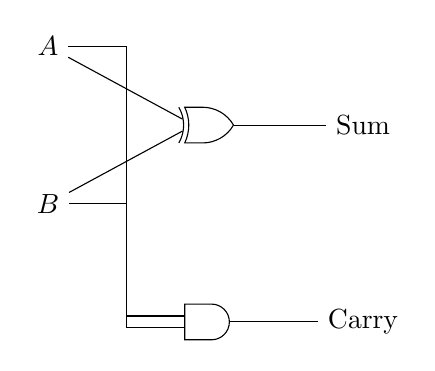
\begin{tikzpicture}[circuit logic US, scale=1, transform shape]

		% Inputs
		\node (A) at (0, 2) {\( A \)};
		\node (B) at (0, 0) {\( B \)};

		% XOR gate
		\node [xor gate US, draw, logic gate inputs=nn] (xor1) at (2, 1) {};
		\draw (A) -- (xor1.input 1);
		\draw (B) -- (xor1.input 2);

		% AND gate
		\node [and gate US, draw, logic gate inputs=nn] (and1) at (2, -1.5) {};
		\draw (A) -- ++(1,0) |- (and1.input 1);
		\draw (B) -- ++(1,0) |- (and1.input 2);

		% Outputs
		\node (Sum) at (4, 1) {\( \text{Sum} \)};
		\node (Carry) at (4, -1.5) {\( \text{Carry} \)};
		\draw (xor1.output) -- (Sum);
		\draw (and1.output) -- (Carry);

	\end{tikzpicture}
\end{center}

The XOR gate produces the sum bit, while the AND gate produces the carry bit. This forms the fundamental building block of a full binary adder.

\section{Adding Two Single-Byte Binary Numbers Using XOR and AND}

Binary addition can be performed on two single-byte numbers using bitwise operations. Specifically:
- The \textbf{XOR (Exclusive OR)} operation gives the sum of two bits without considering the carry.
- The \textbf{AND} operation identifies where a carry will occur.
- The carry is then shifted left by one position and added to the result in subsequent iterations.

\textbf{Algorithm:}
1. Compute the sum without carry using XOR:
   \[
   \text{sum} = a \oplus b
   \]
2. Compute the carry using AND and shift it left by one bit:
   \[
   \text{carry} = (a \land b) \ll 1
   \]
3. Repeat the process by adding the carry to the sum until there is no carry left.

\textbf{Diagram:}
Below is a diagram that illustrates the process for a single bit addition.

\begin{center}
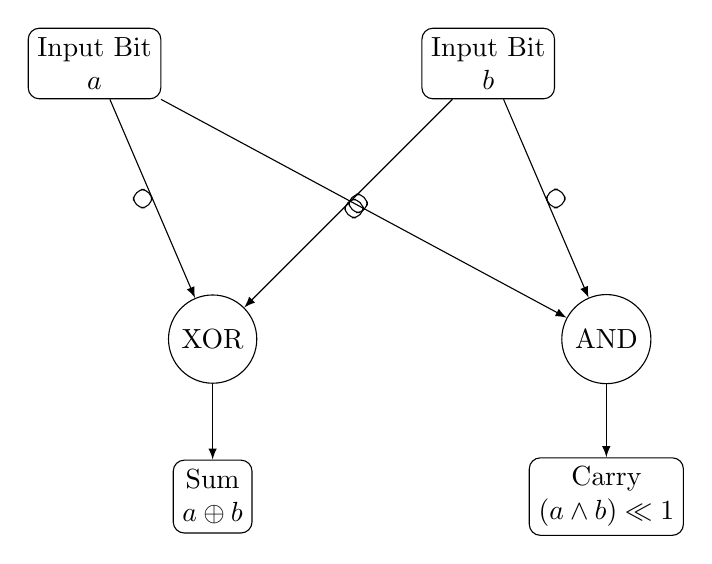
\begin{tikzpicture}[node distance=2cm, every node/.style={draw, rectangle, rounded corners, align=center}]
    % Nodes
    \node (A) {Input Bit \\ $a$};
    \node (B) [right of=A, xshift=3cm] {Input Bit \\ $b$};
    \node (XOR) [below of=A, yshift=-1.5cm, xshift=1.5cm, draw, circle] {XOR};
    \node (SUM) [below of=XOR] {Sum \\ $a \oplus b$};
    \node (AND) [right of=XOR, xshift=3cm, draw, circle] {AND};
    \node (CARRY) [below of=AND] {Carry \\ $(a \land b) \ll 1$};

    % Arrows
    \draw[->] (A) -- (XOR) node[midway, left] {};
    \draw[->] (B) -- (XOR) node[midway, right] {};
    \draw[->] (XOR) -- (SUM);
    \draw[->] (A) -- (AND) node[midway, left] {};
    \draw[->] (B) -- (AND) node[midway, right] {};
    \draw[->] (AND) -- (CARRY);
\end{tikzpicture}
\end{center}

\textbf{Example:}
Consider two single-byte binary numbers:
\[
a = 01101101, \quad b = 10101001
\]

1. Compute the XOR for the sum:
   \[
   \text{sum} = a \oplus b = 11000100
   \]

2. Compute the AND for the carry and shift left:
   \[
   \text{carry} = (a \land b) \ll 1 = 00001010
   \]

3. Add the sum and carry:
   - New sum: \( \text{sum} = 11000100 \oplus 00001010 = 11001110 \)
   - New carry: \( \text{carry} = (11000100 \land 00001010) \ll 1 = 00000000 \)

4. Final result: \( 11001110 \).

\end{document}
